\chapter{Hardware Detail Design}
\label{chap:5}

This chapter gives a detailed discussion on the hardware design and
configuration of this system. This includes the relay switching circuit, the
motor and coil design and the NFC chip configuration.

See Appendix \ref{app:d} for a schematic layout of the hardware and their
connections.

\section{Relay Switch Circuit}
\label{sec:detail-switch}

As explained in Sec. \ref{sec:relay-switch} on p.\pageref{sec:relay-switch}, a relay
switch [\cite{manual:relay-specs}], in conjunction with a 2N2222
Bipolar Junction Transistor (BJT) [\cite{maunual:transistor-datasheet}], is used
by the Raspberry Pi to control the motor. See Fig.
\ref{fig:relay-switch} for the circuit diagram.

\begin{figure}
\centering
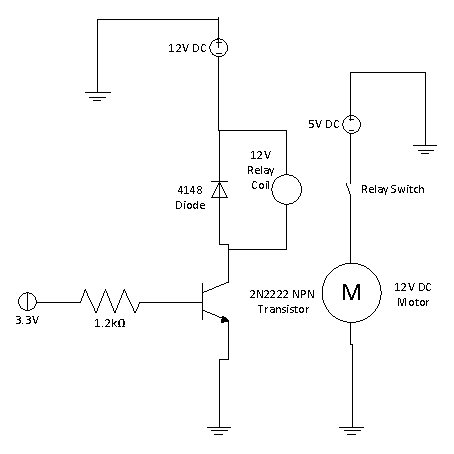
\includegraphics[clip = true, trim = 70 640 0 70, scale=1.2]{relay_switch}
\caption{12 V relay transistor switch.}
\label{fig:relay-switch}
\end{figure}

For the following equations, P$_r$ and V$_r$ is the power dissipation in the relay coil
and voltage across the relay coil, $\beta$ is the BJT current amplification, V$_p$ and
I$_p$ is the voltage and current supply from a Raspberry Pi's GPIO pin and I$_b$ and
R$_b$ is the BJT's base current and resistor.

The relevant  parameters for these components are [\cite{manual:relay-specs},
\cite{maunual:transistor-datasheet}]:

\[ \mathrm{\ P_{r}} = 0.36\mathrm{\ W}\]
\[ \mathrm{\ V_{r}} = 12\mathrm{\ V}\]
\[ \mathrm{\ \beta} \approx 10\]
\[ \mathrm{\ V_{p}} = 3.3\mathrm{\ V}\]

From the relay's power dissipation and voltage, its current draw is found by

\[
\mathrm{\ I_{r}} = \frac{\mathrm{\ P_{r}}}{\mathrm{\ V_{r}}}
\]

which gives a current draw of

\[
\mathrm{\ I_{r}} = 0.03\mathrm{\ A}
\]

Taking the BJT's current amplification as roughly 10, as recommended by the
BJT's datasheet [\cite{maunual:transistor-datasheet}], the current draw from the
Pi to the base of the BJT is given by

\[
\mathrm{\ I_{b}} = \frac{\mathrm{\ I_{r}}}{\beta}
\]

This gives a current draw of

\[
\mathrm{\ I_{b}} = 3\mathrm{\ mA}
\]

The maximum allowable current draw from a GPIO pin is 16 mA
[\cite{website:gpio-specs}], though this is not recommended as the Pi does not
have any current limiting or over-current protection hardware. A current draw of 5mA per
pin is recommended by the Pi's manufacturers [\cite{website:gpio-specs}]. Therefore, a
current draw of 3 mA is completely safe.

To limit the current draw from the Pi, a base resistor must be added between the Pi's GPIO pin
and the BJT's base. With a current draw of 3 mA and a voltage of 3.3 V, the
resistor size is found by using Ohm's law:

\[
\mathrm{\ R_{b}} = \frac{\mathrm{\ V_{p}}}{\mathrm{\ I_{p}}}
\]

which gives

\[
\mathrm{\ R_{b}} = 1.1\mathrm{\ k\Omega}
\]

To prevent voltage spikes from the Pi's GPIO's from supplying to much current, a
further 10\% was added to the resistor size. This gives a resistor size of

\[\mathrm{\ R_{b}} = 1.2\mathrm{\ k\Omega}\]

which draws a current of 

\[\mathrm{\ I_{b}} = 2.75\mathrm{\ mA} \]

which is still enough to activate the relay's coil and turn the motor on. 

\section{NFC Chip}

The Near Field Communication (NFC) chip used, is the Adafruit NFC shield for an
Arduino Uno microcontroller [\cite{website:adafruit-nfc}]. See Sec.
\ref{sec:nfc-controller} on p.\pageref{sec:nfc-controller} for more details
on the controller.

The shield was designed and built to be used by an Arduino Uno microcontroller.
Therefore, some modification to the chip's connections had to be made before it
was able to communicate with the Pi. By default, the chip was made to communicate with an
Arduino using the Inter Integrated Circuit (i$^2$c) communication protocol. However, the
component manufacturers have added connection pads to the chip that, when shorted, allows
the chip to communicate via Serial Peripheral Interface (SPI) or Transistor
Transistor Login (TTL). The libnfc library is currently only configured to allow
communication via an Universal Asynchronous Receiver Transmitter (UART). Therefore, the
chip was modified to communicate via its TTL interface, which is compatible with the Pi's
UART interface. 

See Appendix \ref{app:nfc-chip-config} for detailed explanation on this
configuration process and also how the libnfc library was built and compiled. 

\section{Vending Machine Unit}

A small VM unit was constructed for demonstration purposes. It is
designed to house all the VM components, i.e. the two DC motors,
the two coils, the Raspberry Pi central controller, the NFC shield and the
webcam.

Four 10 mm vent holes were added at the sides to improve air circulation
and to provide external wire access, while a larger 60 mm vent hole was also
added to allow for an external 60 mm desktop computer fan to be added at a
later stage.

The unit is made from 1.6 mm thick mild steel and the components were cut and
bent by Fabrinox, Paarl and welded together by the Electrical and Electronic
Engineering Department of Stellenbosch University's workshop.

See Fig. \ref{fig:vm-actual} in Appendix \ref{app:vm-tekeninge} for a picture of the
complete VM unit with the two DC motor inserted. See Appendix \ref{app:vm-tekeninge} for
detailed design drawings of the VM unit.

\section{Webcam}

As discussed in Sec. \ref{sec:webcam}, a Sony PS2 Eye Toy  webcam was
attached to the Raspberry Pi. This allows the VM to scan a live
video feed for a QR Code. It is already compatible with the Raspberry Pi and
therefore requires minimal configuration to begin working.

It is important to note that a Raspbian version from early 2013 was used on the
Raspberry Pi. It was found that the latest Raspbian distributions have an
unknown bug in its Video4Linux video drivers which causes the EyeToy to
work incorrectly. Furthermore, the camera needs to be plugged into a Universal Serial Bus
(USB) port on the Pi itself and not into an external USB hub. This is done to prevent
hardware timing issues that are introduced when a USB hub is used.

\section{Motor and Coil}

The VM dispenses products by activating a motor that turns a coil
loaded with a product. This turning motion causes a product to move along the
coil in an Archimedean screw-like manner until it falls off at the end of the
coil. 

In the demonstration VM, two coils are used. The coils are made
from 2.5 mm thick galvanised iron wire. The coil diameter is 50 mm and has a
longitudinal pitch of 20 mm. 

It is important to only activate the motor for one turn of the coil to
ensure that only one product is dispensed per completed transaction. This is
currently being done by only activating a motor for a set amount of time. To
determine this time, it was required that the speed of the motor be
determined for a given supply voltage. The motors that are used are 12 V DC motors made
by Faulhaber [\cite{manual:dc-motors}] coupled with a 14:1 speed gearbox
[\cite{manual:gearbox}].

For the following calculations, V$_o$, I and R are the motor supply voltage, current and
terminal resistance, V$_e$ is the back-Electromotive Force (EMF) voltage, $\omega$ is
the motor speed and k$_e$ is the Back-EMF constant.

The following equation gives the relationship between a DC motor's supply
voltage and its back-Electromotive Force (EMF) [\cite{article:motor-calc}].

\[ \mathrm{V}_o = \mathrm{IR} + \mathrm{V}_e\]

The back-EMF is proportional to the rotational speed of the motor. Therefore,
the V$_e$ term can be taken as

\[ \mathrm{V}_e = \mathrm{k}_e\omega\]

which gives the following equation

\begin{equation}
 \label{eq:motor}
 \mathrm{V}_o = \mathrm{IR} + \mathrm{k}_e\omega
\end{equation}

The IR term is taken as constant, since the torque load on the motor stays the constant.
From the motor's datasheets and usage tests, the I, R and k$_e$ terms were
determined to have the following values:

\[\mathrm{I} = 0.35\mathrm{\ A}\]
\[\mathrm{R} = 0.41\mathrm{\ \Omega}\]
\[ \mathrm{k}_e = 2 \mathrm{\ mV/rpm}\]

Using these values, and setting the input voltage as 3.3 V in equation
\ref{eq:motor}, the motor's speed was determined to be 113 RPM. Therefore, to
complete a single revolution, the motor may only be activated for 0.53 seconds. 

This is not the most effective method, however, because the errors in the system
accumulate over time. In time, these errors may lead incorrect product
dispensing. 

To improve this, a proximity sensor may be added onto the coil and onto the
VM wall. This sensor can be connected to and be controlled by the
Raspberry Pi and would be activated every time the coil completes one
revolution. When the sensor is triggered, the Pi will then know that exactly
one revolution has been completed and stop the motor. This will stop any errors
from accumulating over time and make the VM more reliable. 
